\documentclass{beamer}
%\documentclass[aspectratio=169]{beamer}  % inna proporcja slajdu

\usepackage[utf8]{inputenc}
\usepackage{polski}
\usepackage{amsmath}
\usepackage{amssymb}
\usepackage{mathtools}
\usepackage{mathabx}

\usetheme{pwrlite}
%\usetheme[nosections]{pwrlite}  % wyłączenie stron z sekcjami
%\usetheme[en]{pwrlite}  % logo w wersji angielskiej
%\usetheme[nosections,en]{pwrlite}  % logo w wersji angielskiej i bez sekcji

%\pdfmapfile{+lato.map}  % jeśli nie działa font Lato (a jest zainstalowany), odkomentuj przy pierwszej kompilacji

\title{Ewolucyjny algorytm dla nieliniowego zadania transportowego}
\institute{Wydział Podstawowych Problemów Techniki}
\author{Piotr Berezowski}
% \date{5 lutego 2019}

\begin{document}

\begin{frame}
\frametitle{Plan prezentacji}
\begin{itemize}
\item Cel pracy
\item Wprowadzenie
    \begin{itemize}
    \item Zadanie transportowe
    \item Algorytmy ewolucyjne
    \end{itemize}
\item Implementacja
\item Wersja równoległa    
\item Wyniki
\item Podsumowanie
\end{itemize}
\end{frame}

\section{Wprowadzenie}

\begin{frame}
\frametitle{Cel pracy}
\begin{enumerate}
    \item Implementacja algorytmu ewolucyjnego dla zadania transportowego.
    \item Analiza eksperymentalna.
\end{enumerate}
\end{frame}

\begin{frame}
\frametitle{Zadanie transportowe}
\only<1> {
    \begin{itemize}
        \item Mamy zdefiniowane $n$ punktów nadania i $m$ punktów odbioru.
        \item Każdy z punktów nadania ma określoną podaż.
        \item Każdy punkt odbioru ma określony popyt.
        \item Znaleźć plan optymalnego transportu.
    \end{itemize}
}
\only<2> {
    Funkcja celu:
    $$\min \sum_{i=1}^{n} \sum_{j=1}^{m} f_{ij}(x_{ij})$$
    Ograniczenia:
    $$\sum_{j=1}^{m} x_{ij} = supply(i), \text{ dla } i = 1, 2, \dots, n$$
    $$\sum_{i=1}^{n} x_{ij} = demand(j), \text{ dla } j = 1, 2, \dots, m$$
    $$x_{ij} \ge 0, \text{ dla } i = 1, 2, \dots, n \text{ i } j = 1, 2, \dots, m$$
}
\end{frame}

\begin{frame}
\frametitle{Algorytmy ewolucyjne}
\only<1> {
    \begin{itemize}
        \item Są podzbiorem algorytmów metaheurystycznych.
        \item Inspirowane teorią ewolucji Darwina.
        \item Populacja rozwiązań ewoluuje tworząc coraz lepsze rozwiązania.
    \end{itemize}
}
\only<2> {
    \begin{figure}[H]
        \centering        
        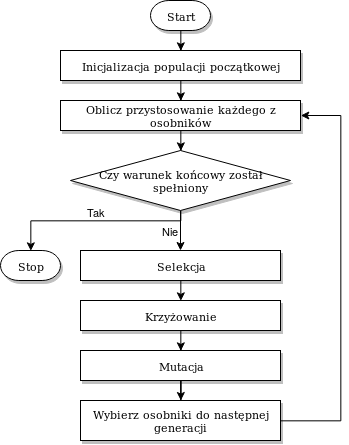
\includegraphics[width=0.5\textwidth]{alg_gen_szkic.png}
        % \caption{Ogólny schemat działania algorytmu ewolucyjnego}
        \label{alg_ewo_img}
    \end{figure}
}
\end{frame}

\section{Implementacja}

\begin{frame}
\frametitle{Implementacja}
\only<1> {
    \begin{itemize}
        \item Reprezentacja rozwiązania w postaci macierzy.
        \item Najbardziej intuicyjny sposób reprezentacji dla omawianego problemu.
    \end{itemize}
    \begin{table}
        \begin{center}
            \begin{tabular}{c||ccccc||c}
                & $s_1$ & $s_2$ & $s_3$ & $s_4$ & $s_5$ & $demand$ \\ 
                \hline
                \hline
                $d_1$ & 0.0 & 7.0 & 5.0 & 0.0 & 0.0 & 12.0 \\
                $d_2$ & 5.0 & 0.0 & 0.0 & 0.0 & 5.0 & 10.0 \\
                $d_3$ & 3.0 & 0.0 & 0.0 & 0.0 & 0.0 & 3.0 \\
                $d_4$ & 0.0 & 0.0 & 0.0 & 3.0 & 7.0 & 10.0 \\
                $d_5$ & 2.0 & 0.0 & 0.0 & 10.0 & 0.0 & 12.0 \\
                \hline
                \hline
                $supply$ & 10.0 & 7.0 & 5.0 & 13.0 & 12.0 & \\ 
            \end{tabular}
        \end{center}
        \caption{Przykładowe rozwiązanie.}
    \end{table}
}

\only<2> {
    Inicjalizacja:
    \begin{itemize}
        \item Generujemy losową permutację wszystkich indeksów macierzy rozwiązania.
        \item Wstawiamy po kolei dla komórki o indeksie $(i, j)$ $val = \min(demand[i], supply[j])$.
        \item Zmniejszamy odpowiednio popyt i podaż o wartość $val$. 
    \end{itemize}
}

\only<3-8> {
    Przykład:
    \begin{itemize}
        \item Macierz $2 \times 3$
        \item Permutacja indeksów: $[(2,1),(1,3),(2,3),(2,2),(1,2),(1,1)]$
    \end{itemize}
}
\only<3> {
    \begin{table}
        \begin{center}
            \begin{tabular}{c||ccc||c}
                & $s_1$ & $s_2$ & $s_3$ & $demand$ \\ 
                \hline
                \hline
                $d_1$ & 0.0 & 0.0 & 0.0 & 8.0 \\
                $d_2$ & 0.0 & 0.0 & 0.0 & 12.0 \\
                \hline
                \hline
                $supply$ & 5.0 & 8.0 & 7.0 & \\ 
            \end{tabular}
        \end{center}
        \caption{Niezainicjalizowana macierz}
    \end{table}
}

\only<4> {
    % (2,1)
    \begin{table}
        \begin{center}
            \begin{tabular}{c||ccc||c}
                & $s_1$ & $s_2$ & $s_3$ & $demand$ \\ 
                \hline
                \hline
                $d_1$ & 0.0 & 0.0 & 0.0 & 8.0 \\
                $d_2$ & \textbf{5.0} & 0.0 & 0.0 & \textbf{7.0} \\
                \hline
                \hline
                $supply$ & \textbf{0.0} & 8.0 & 7.0 & \\ 
            \end{tabular}
        \end{center}
        \caption{Inicjalizujemy indeks $(2,1)$}
    \end{table}
}

\only<5> {
    % (2,1), (1,3)
    \begin{table}
        \begin{center}
            \begin{tabular}{c||ccc||c}
                & $s_1$ & $s_2$ & $s_3$ & $demand$ \\ 
                \hline
                \hline
                $d_1$ & 0.0 & 0.0 & \textbf{7.0} & \textbf{1.0} \\
                $d_2$ & 5.0 & 0.0 & 0.0 & 7.0 \\
                \hline
                \hline
                $supply$ & 0.0 & 8.0 & \textbf{0.0} & \\ 
            \end{tabular}
        \end{center}
        \caption{Inicjalizujemy indeks $(1,3)$}
    \end{table}
}

\only<6> {
    % (2,1), (1,3), (2,3)
    \begin{table}
        \begin{center}
            \begin{tabular}{c||ccc||c}
                & $s_1$ & $s_2$ & $s_3$ & $demand$ \\ 
                \hline
                \hline
                $d_1$ & 0.0 & 0.0 & 7.0 & 1.0 \\
                $d_2$ & 5.0 & 0.0 & \textbf{0.0} & \textbf{7.0} \\
                \hline
                \hline
                $supply$ & 0.0 & 8.0 & \textbf{0.0} & \\ 
            \end{tabular}
        \end{center}
        \caption{Inicjalizujemy indeks $(2,3)$}
    \end{table}
}

\only<7> {
    % (2,1), (1,3), (2,3), (2,2)
    \begin{table}
        \begin{center}
            \begin{tabular}{c||ccc||c}
                & $s_1$ & $s_2$ & $s_3$ & $demand$ \\ 
                \hline
                \hline
                $d_1$ & 0.0 & 0.0 & 7.0 & 1.0 \\
                $d_2$ & 5.0 & \textbf{7.0} & 0.0 & \textbf{0.0} \\
                \hline
                \hline
                $supply$ & 0.0 & \textbf{1.0} & 0.0 & \\ 
            \end{tabular}
        \end{center}
        \caption{Inicjalizujemy indeks $(2,2)$}
    \end{table}
}

\only<8> {
    % (2,1), (1,3), (2,3), (2,2), (1,2)
    \begin{table}
        \begin{center}
            \begin{tabular}{c||ccc||c}
                & $s_1$ & $s_2$ & $s_3$ & $demand$ \\ 
                \hline
                \hline
                $d_1$ & 0.0 & \textbf{1.0} & 7.0 & \textbf{0.0} \\
                $d_2$ & 5.0 & 7.0 & 0.0 & 0.0 \\
                \hline
                \hline
                $supply$ & 0.0 & \textbf{0.0} & 0.0 & \\ 
            \end{tabular}
        \end{center}
        \caption{Inicjalizujemy indeks $(1,2)$}
    \end{table}
}

\only<9> {
    \begin{itemize}
        \item Operator krzyżowania
            \begin{itemize}
                \item Selekcja metodą ruletki.
                \item Kombinacja wypukła dwóch rodziców.
                \item Ograniczenia zadania są spełnione przez dzieci, jeśli są spełnione przez rodziców.
            \end{itemize}
        \item Operator mutacji
            \begin{itemize}
                \item Wybieramy losową podmacierz z macierzy rozwiązania.
                \item Inicjalizujemy na nowo podmacierz. 
            \end{itemize}
    \end{itemize}
}
    
\end{frame}

\section{Wersja równoległa}

\begin{frame}
    \frametitle{Modele ewolucji}
    Dodano dwa modele ewolucji populacji:
    \begin{itemize}
        \item Klasyczny
        \begin{itemize}
            \item Zrównoleglenie na poziomie operatorów i funkcji przystosowania.
        \end{itemize}
        \item Wyspowy
        \begin{itemize}
            \item Podział na populacje częściowe.
            \item Każda populacja ewoluuje niezależnie od innych przez określoną liczbę pokoleń.
        \end{itemize}
    \end{itemize}
\end{frame}


\section{Wyniki}

\begin{frame}
\frametitle{Czas znalezienia rozwiązania}
\begin{figure}[ht]
    \centering
    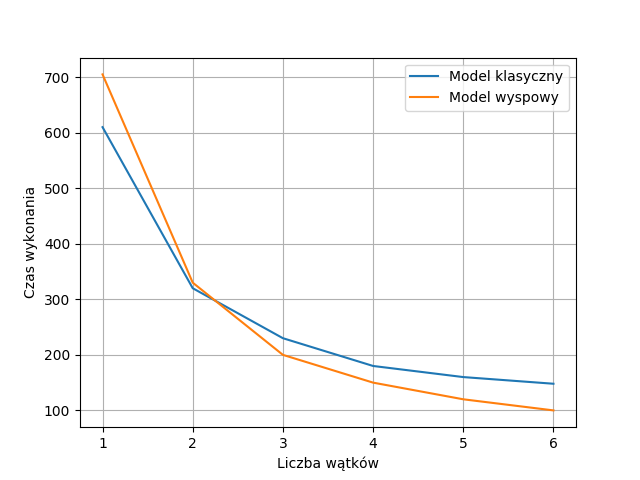
\includegraphics[scale=0.5]{time_threads_compare.png}
    \caption{Zależność czasu znalezienia rozwiązania od liczby wątków}
\end{figure}    
\end{frame}

\begin{frame}
    \frametitle{Funkcja liniowa}
    \only<1> {
        \begin{table}
            \begin{center}
                \begin{tabular}{c||c|c|c|c}
                    Rozmiar zadania & GLPK & Ipopt & Klasyczny & Wyspowy \\ 
                    \hline
                    $7\times7$ & 293.0 & 292.9 & 490.5 & 292.9 \\
                \end{tabular}
            \end{center}
            \caption{Rezultaty}
        \end{table}
    }

    \only<2> {
        \begin{figure}[ht]
            \centering
            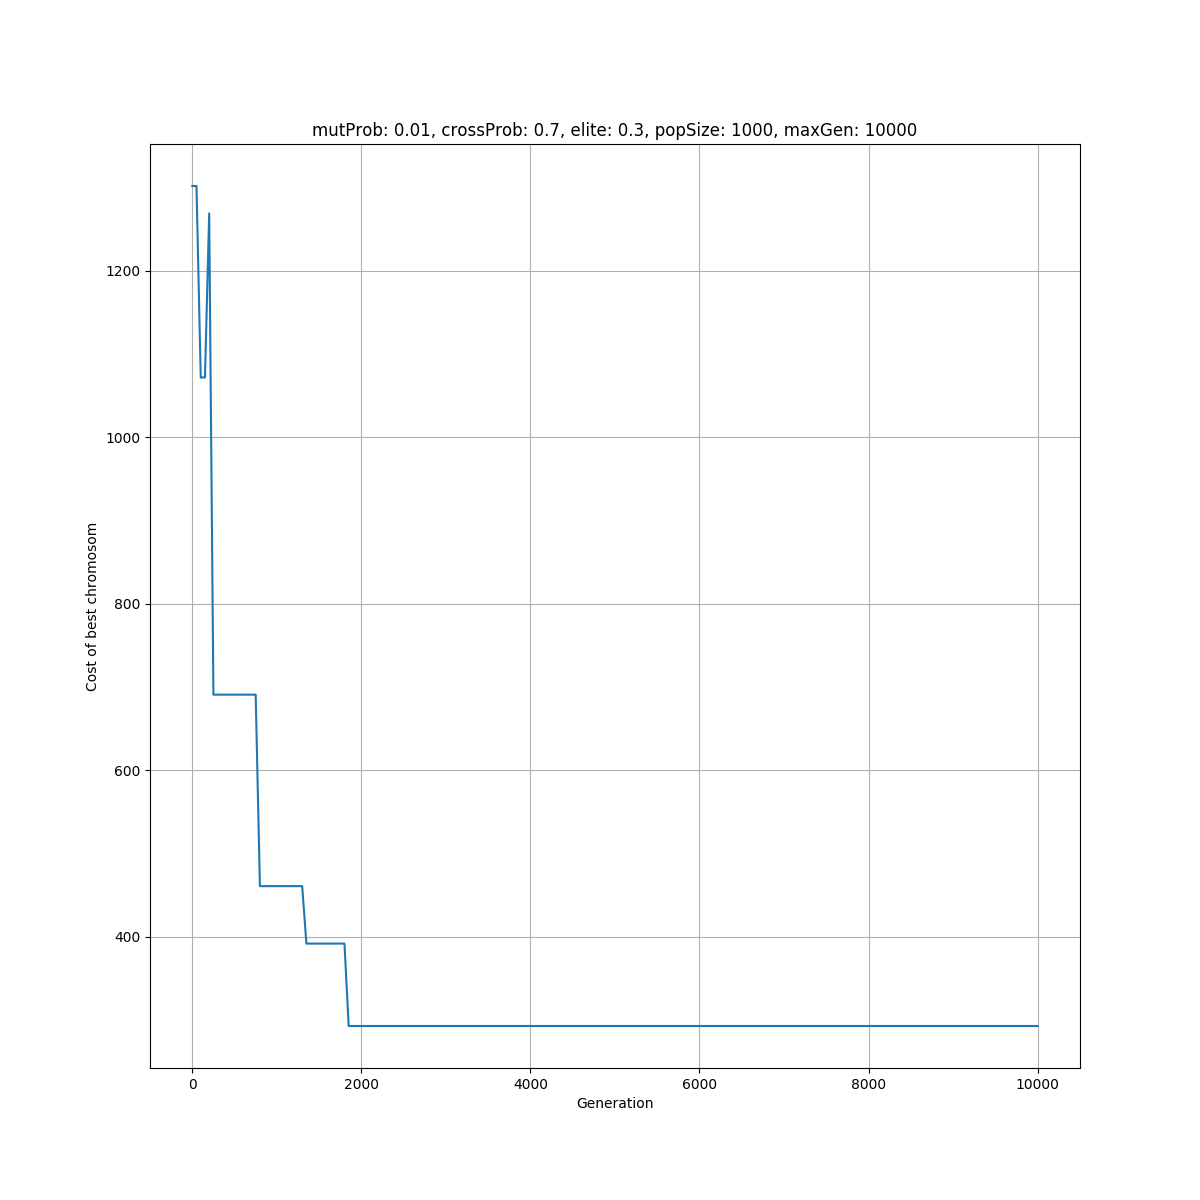
\includegraphics[scale=0.2]{resultPlot_lin_island.png}
            \caption{Ewolucja najlepszego rozwiązania dla modelu wyspowego}
        \end{figure}    
    }
    

\end{frame}

\begin{frame}
    \frametitle{Funkcja nieliniowa}
    \only<1> {
        \begin{table}
            \begin{center}
                \begin{tabular}{c||c|c}
                    Rozmiar zadania & Klasyczny & Wyspowy \\ 
                    \hline
                    $7\times7$ & 62.0 & 0.0 \\
                \end{tabular}
            \end{center}
            \caption{Rezultaty}
        \end{table}
    }
    
    \only<2> {
        \begin{figure}[ht]
            \centering
            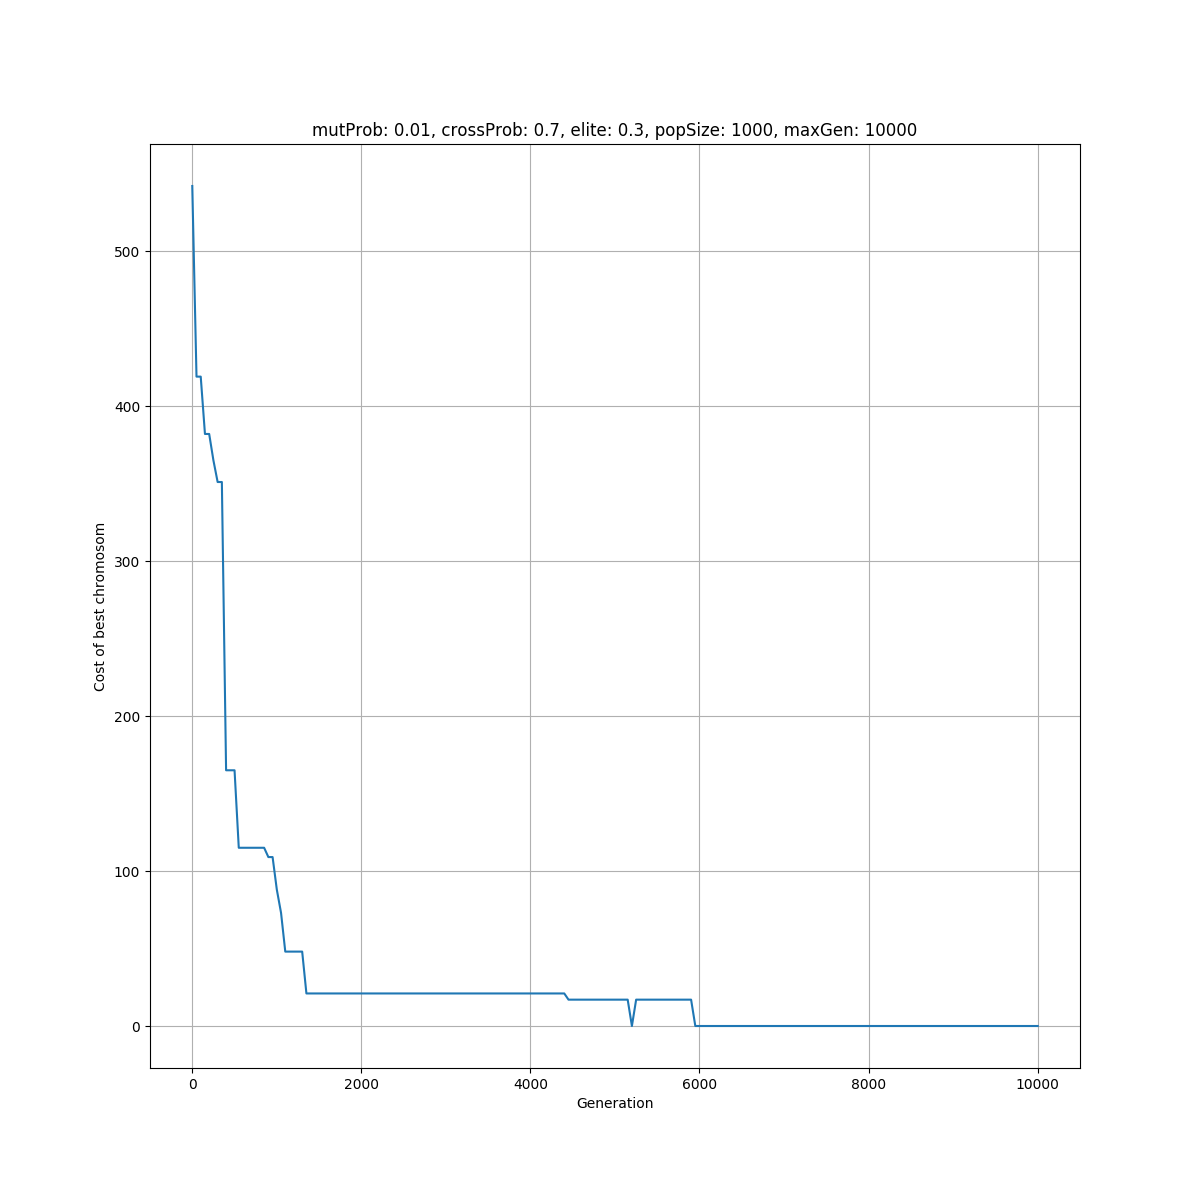
\includegraphics[scale=0.2]{resultPlot_island.png}
            \caption{Ewolucja najlepszego rozwiązania dla modelu wyspowego}
        \end{figure}
    }

    \only<3> {
        \begin{figure}[ht]
            \centering
            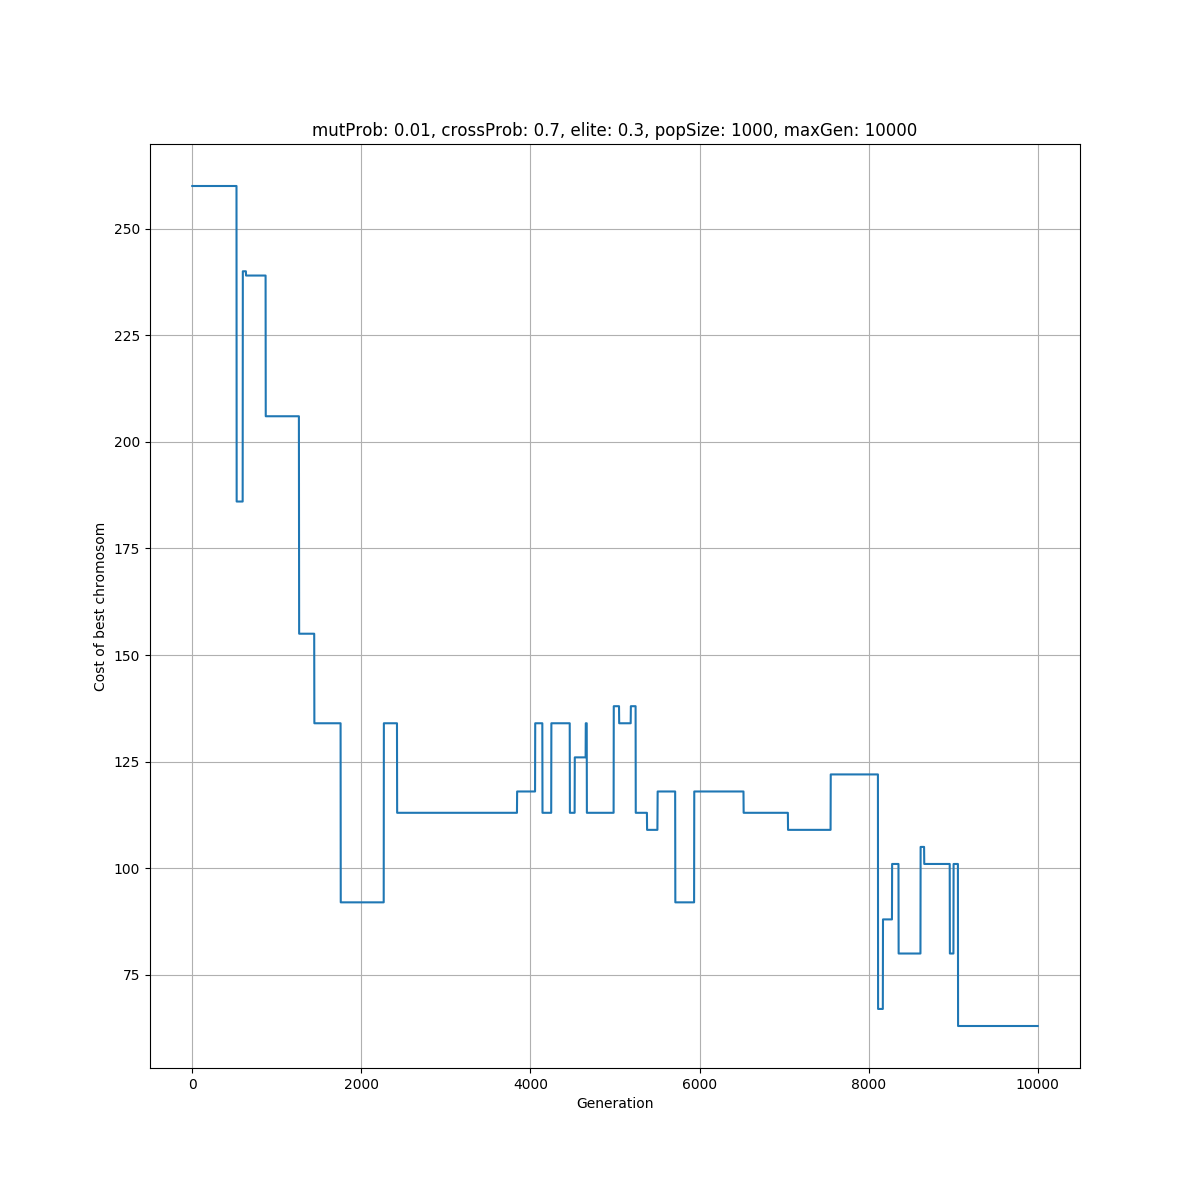
\includegraphics[scale=0.2]{resultPlot_regular.png}
            \caption{Ewolucja najlepszego rozwiązania dla modelu klasycznego}
        \end{figure}
    }
    

\end{frame}

\section{Podsumowanie}

% \begin{frame}
% \frametitle{Bibliografia}
% \bibliographystyle{bibliografia_styl.bst}
% \bibliography{bibliografia.bib}
% \end{frame}

\end{document}

